\documentclass[11pt,a4paper]{article}

\usepackage[utf8]{inputenc}
\usepackage[T1]{fontenc}
\usepackage{mathpazo}
\usepackage[scaled=0.92]{helvet}
\usepackage[margin=1in]{geometry}
\usepackage{graphicx}
\usepackage{amsmath,amssymb,amsfonts}
\usepackage{booktabs}
\usepackage{tabularx}
\usepackage{setspace}
\usepackage{titlesec}
\usepackage{fancyhdr}
\usepackage{float}
\usepackage{caption}
\usepackage{microtype}

\usepackage{tikz}
\usetikzlibrary{shapes.geometric, arrows.meta, positioning, calc, shadows, backgrounds}

\usepackage{tcolorbox}
\usepackage[hidelinks]{hyperref}

\setstretch{1.15}
\setlength{\parindent}{0pt}
\setlength{\parskip}{0.8em}
\sloppy

\titleformat{\section}{\normalfont\large\bfseries\sffamily}{\thesection}{1em}{}
\titleformat{\subsection}{\normalfont\normalsize\bfseries\sffamily}{\thesubsection}{1em}{}

\pagestyle{fancy}
\fancyhf{}
\fancyhead[L]{\small\sffamily Fondasi Basis Data: Model Relasional}
\fancyhead[R]{\small\sffamily\thepage}
\renewcommand{\headrulewidth}{0.4pt}

\captionsetup{font=small,labelfont=bf,labelsep=period}

\newtcolorbox{skema}[1][]{
	colback=gray!5,
	colframe=gray!40,
	boxrule=0.5pt,
	arc=3pt,
	fontupper=\small\sffamily,
	title=#1,
	coltitle=black,
	attach boxed title to top left={yshift=-2mm, xshift=5mm},
	boxed title style={colback=white, boxrule=0.5pt, arc=2pt}
}

\renewenvironment{abstract}
{\small
	\begin{center}\textbf{\sffamily Abstract}\end{center}
	\begin{quote}}
	{\end{quote}}

\title{\vspace{-1.5cm}\textbf{\sffamily\LARGE Model Relasional:\\ Fondasi Penyimpanan Data Modern dan Transformasi ERD ke Tabel}}
\author{
	\textbf{Muhammad Riduwan Khafidi} \\
	\small Program Studi Teknik Rekayasa Perangkat Lunak \\
	\small Politeknik Negeri Batam \\
	\small \texttt{4342611034@students.polibatam.ac.id}
}
\date{\small\today}

\begin{document}

\maketitle
\thispagestyle{empty}

\begin{abstract}
	Model relasional yang diperkenalkan oleh Edgar F. Codd pada tahun 1969 merupakan tonggak sejarah dalam pengelolaan basis data. Model ini merevolusi cara data disimpan dan diakses dengan memetakan seluruh informasi ke dalam bentuk tabel dua dimensi yang sederhana, namun memiliki landasan matematis yang kuat. Makalah ini membedah secara komprehensif konsep dasar model relasional, mulai dari sejarah, definisi, terminologi formal (seperti relasi, tuple, dan atribut), karakteristik tabel yang valid, hingga hirarki kunci (keys) yang menjamin integritas data. Bagian utama makalah ini berfokus pada panduan sistematis untuk menerjemahkan skema konseptual (Entity Relationship Diagram) menjadi skema fisik (Relational Schema). Pembahasan mencakup pemetaan entitas, relasi (one-to-one, one-to-many, many-to-many), atribut multivalued, agregasi, hingga strategi penanganan spesialisasi (inheritance).
\end{abstract}

\section{Pendahuluan: Revolusi Edgar F. Codd}

Dalam alur perancangan basis data, setelah kita berhasil memetakan kebutuhan pengguna ke dalam model konseptual (seperti ERD atau EERD), tahap selanjutnya adalah menerjemahkannya ke dalam model fisik. Di sinilah Model Relasional berperan. Dirumuskan pertama kali oleh Edgar F. Codd (seorang ilmuwan komputer di IBM) pada tahun 1969, model ini mengubah cara pandang dunia terhadap basis data.

Sebelum adanya model relasional, basis data dikelola menggunakan model hierarkis atau jaringan yang sangat rumit. Codd mengajukan pendekatan yang jauh lebih elegan: seluruh data diwakili dalam bentuk tabel dua dimensi (yang secara matematis disebut sebagai \textit{relations}). Pendekatan ini tidak hanya memudahkan para programmer dalam melakukan operasi manipulasi data (seperti \textit{query}, \textit{update}, dan \textit{delete}), tetapi juga sangat mudah dipahami bahkan oleh kalangan non-programmer karena bentuknya yang intuitif.

\section{Terminologi Dasar Model Relasional}

Meskipun dalam percakapan sehari-hari kita terbiasa menggunakan istilah "tabel", "baris", dan "kolom", model relasional memiliki terminologi formal yang wajib dipahami. Gambar \ref{fig:terminology} mengilustrasikan padanan antara istilah formal dengan istilah alternatif yang umum digunakan.

\begin{figure}[H]
	\centering
	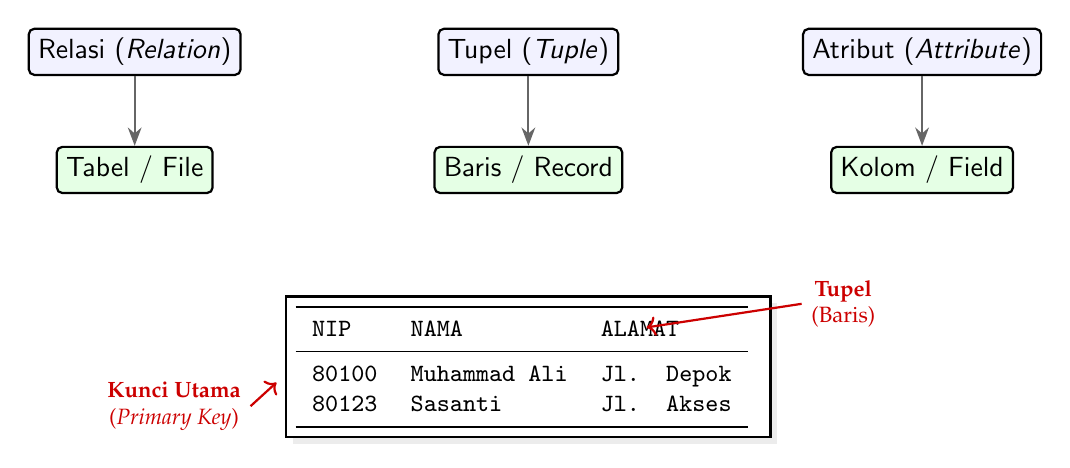
\begin{tikzpicture}[
			box/.style={draw, rectangle, fill=blue!5, thick, align=center, font=\sffamily, rounded corners=2pt},
			arrow/.style={->, >=Stealth, thick, color=gray!80!black}
		]
		% Baris 1: Terminologi
		\node[box] (rel) at (0,0) {Relasi (\textit{Relation})};
		\node[box] (tup) at (5,0) {Tupel (\textit{Tuple})};
		\node[box] (att) at (10,0) {Atribut (\textit{Attribute})};

		% Baris 2: Istilah Alternatif
		\node[box, fill=green!10] (tab) at (0,-1.5) {Tabel / File};
		\node[box, fill=green!10] (row) at (5,-1.5) {Baris / Record};
		\node[box, fill=green!10] (col) at (10,-1.5) {Kolom / Field};

		\draw[arrow] (rel) -- (tab);
		\draw[arrow] (tup) -- (row);
		\draw[arrow] (att) -- (col);

		% Contoh Tabel
		\node[draw, rectangle, align=left, font=\small\ttfamily, fill=white, thick, drop shadow={opacity=0.15}] (table) at (5,-4) {
			\begin{tabular}{l l l}
				\toprule
				\textbf{NIP} & \textbf{NAMA} & \textbf{ALAMAT} \\
				\midrule
				80100        & Muhammad Ali  & Jl. Depok       \\
				80123        & Sasanti       & Jl. Akses       \\
				\bottomrule
			\end{tabular}
		};

		% Anotasi
		\node[font=\footnotesize, text=red!80!black, align=center] (pk) at (0.5,-4.5) {\textbf{Kunci Utama}\\(\textit{Primary Key})};
		\draw[->, red!80!black, thick] (pk.east) -- (1.8,-4.2);

		\node[font=\footnotesize, text=red!80!black, align=center] (tupel) at (9,-3.2) {\textbf{Tupel}\\(Baris)};
		\draw[->, red!80!black, thick] (tupel.west) -- (6.5,-3.5);

	\end{tikzpicture}
	\caption{Terminologi Formal Model Relasional dan Contoh Penerapannya.}
	\label{fig:terminology}
\end{figure}

Secara garis besar, sebuah baris data disebut sebagai \textbf{Tupel}. Kumpulan dari nilai-nilai yang mungkin untuk sebuah atribut (misalnya kode divisi: Div01, Div02) disebut \textbf{Domain}. Jumlah kolom dalam sebuah tabel disebut \textbf{Degree} (Derajat), sedangkan jumlah baris dalam tabel disebut \textbf{Cardinality} (Kardinalitas).

\section{Karakteristik dan Aturan Tabel yang Valid}

Tidak semua tabel bisa disebut sebagai relasi yang valid dalam model ini. Terdapat aturan ketat yang harus dipenuhi. Pertama, setiap sel dalam tabel harus bersifat \textbf{atomik}, yang berarti nilainya tidak boleh dipecah lagi menjadi beberapa bagian. Sebagai contoh, kolom "Alamat" tidak boleh berisi "Jl. Ahmad Yani No. 5, Batam", karena itu terdiri dari beberapa nilai (jalan, nomor, kota). Jika ingin atomik, harus dipisah menjadi kolom Jalan, Nomor, dan Kota.

Kedua, tidak boleh ada dua tupel (baris) yang identik. Ketiga, setiap atribut (kolom) harus memiliki nama yang unik. Keempat, urutan baris maupun kolom tidak memiliki arti khusus (tidak harus tersusun secara khusus).

\section{Hirarki Relational Key}

Untuk memastikan tidak ada data yang duplikat, kita membutuhkan Kunci (\textit{Key}). Dalam model relasional, terdapat hirarki kunci yang penting untuk dipahami:

Sebuah \textbf{Super Key} adalah satu atau kumpulan atribut yang secara unik dapat mengidentifikasi sebuah tupel. Dari super key ini, kita memilih yang paling minimal (tanpa atribut yang mubazir) yang disebut \textbf{Candidate Key}. Dari beberapa kandidat, kita memilih satu yang paling utama sebagai \textbf{Primary Key} (Kunci Utama). Sisa kandidat yang tidak terpilih disebut sebagai \textbf{Alternate Key}. Terakhir, sebuah atribut yang menjadi Primary Key di tabel lain, namun hanya menjadi atribut biasa di tabel ini, disebut sebagai \textbf{Foreign Key} (Kunci Tamu).

\section{Transformasi ER-Diagram ke Skema Relasional}

Ini adalah inti dari praktikum pertemuan ini. Bagaimana kita mengubah gambar konseptual (ERD) menjadi tabel fisik? Berikut adalah aturan baku yang harus diikuti.

\subsection{Entitas Kuat dan Entitas Lemah}
Setiap entitas kuat (misalnya "Pegawai") langsung diterjemahkan menjadi sebuah tabel, dengan atribut-atributnya menjadi kolom, dan Primary Key-nya menjadi kunci utama tabel tersebut.

Adapun untuk entitas lemah (misalnya "Pembayaran" yang bergantung pada "Pinjaman"), kita membuat satu tabel tersendiri. Primary Key untuk tabel entitas lemah adalah gabungan dari Primary Key entitas kuat ditambah dengan \textit{partial key} (discriminator) miliknya sendiri. Primary Key entitas kuat ini sekaligus berfungsi sebagai Foreign Key.

\subsection{Relasi One-to-Many (1:N) dan One-to-One (1:1)}
Aturan paling efisien untuk relasi One-to-Many adalah dengan menambahkan Primary Key dari sisi "One" sebagai Foreign Key ke tabel di sisi "Many".

Sebagai ilustrasi, perhatikan Gambar \ref{fig:one_to_many}. Terdapat relasi "Manager" antara entitas "Project" dan "Employee", di mana satu Project hanya punya satu Manager, tetapi satu Employee bisa mengelola banyak Project. Maka, kita menambahkan atribut ID Manager (Foreign Key) ke dalam tabel Project.

\begin{figure}[H]
	\centering
	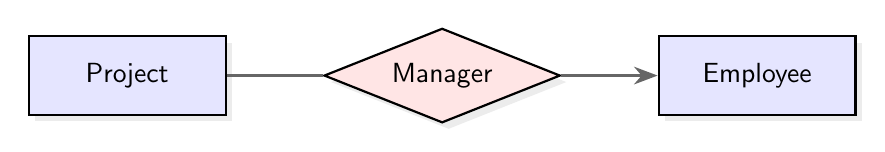
\begin{tikzpicture}[
			entity/.style={draw, rectangle, minimum width=2.5cm, minimum height=1cm, fill=blue!10, thick, font=\sffamily, drop shadow={opacity=0.15}},
			rel/.style={draw, diamond, aspect=2.5, minimum width=3cm, minimum height=1.2cm, fill=red!10, thick, font=\sffamily, drop shadow={opacity=0.15}},
			line/.style={thick, color=gray!80!black}
		]
		\node[entity] (proj) at (-4,0) {Project};
		\node[entity] (emp) at (4,0) {Employee};
		\node[rel] (man) at (0,0) {Manager};

		\draw[line] (proj.east) -- (man.west);
		\draw[line, -{Stealth[length=3mm]}] (man.east) -- (emp.west);
	\end{tikzpicture}
	\caption{Transformasi Relasi One-to-Many menjadi Foreign Key.}
	\label{fig:one_to_many}
\end{figure}

\begin{skema}[Hasil Skema Relasional]
	\textbf{Project} (\underline{P-number}, P-name, Due-Date, \textit{Manager}) \\
	\textbf{Employee} (\underline{SSN}, E-name, Office)
\end{skema}

Jika relasi tersebut memiliki atribut (misalnya tanggal mulai menjadi manager), maka atribut tersebut ikut dipindahkan ke tabel di sisi "One" bersama dengan Foreign Key-nya. Adapun untuk relasi One-to-One, aturannya mirip, kita bebas menaruh Foreign Key di salah satu tabel (biasanya di tabel yang paling sering diakses).

\subsection{Relasi Many-to-Many (M:N)}
Relasi Many-to-Many tidak bisa diselesaikan hanya dengan menambah Foreign Key di salah satu tabel. Kita \textbf{wajib membuat tabel baru} (sering disebut tabel asosiasi/junction). Tabel baru ini setidaknya memiliki dua kolom yang merupakan Foreign Key dari kedua entitas yang dihubungkan, dan kedua kolom tersebut dijadikan satu kesatuan sebagai Primary Key komposit.

Sebagai contoh, pada relasi "Assignment" antara Project dan Employee, kita buat tabel baru bernama Assignment.

\begin{figure}[H]
	\centering
	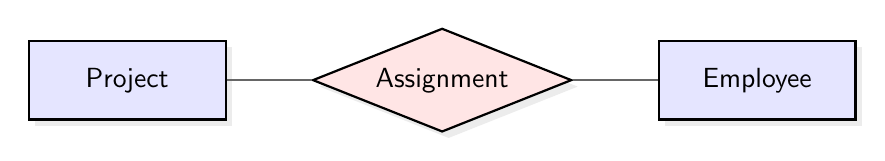
\begin{tikzpicture}[
			entity/.style={draw, rectangle, minimum width=2.5cm, minimum height=1cm, fill=blue!10, thick, font=\sffamily, drop shadow={opacity=0.15}},
			rel/.style={draw, diamond, aspect=2.5, minimum width=3cm, minimum height=1.2cm, fill=red!10, thick, font=\sffamily, drop shadow={opacity=0.15}},
			line/.style={thick, color=gray!80!black}
		]
		\node[entity] (proj) at (-4,0) {Project};
		\node[entity] (emp) at (4,0) {Employee};
		\node[rel] (assign) at (0,0) {Assignment};
		\draw[line] (proj.east) -- (assign.west);
		\draw[line] (assign.east) -- (emp.west);
	\end{tikzpicture}
	\caption{Pembuatan Tabel Baru untuk Relasi Many-to-Many.}
	\label{fig:many_to_many}
\end{figure}

\begin{skema}[Hasil Skema Relasional]
	\textbf{Project} (\underline{P-number}, P-name, Due-Date) \\
	\textbf{Employee} (\underline{SSN}, E-name, Office) \\
	\textbf{Assignment} (\underline{P-number}, \underline{SSN})
\end{skema}

\subsection{Atribut Multivalued dan Komposit}
Atribut yang memiliki lebih dari satu nilai (seperti "Nomor Telepon" pada Pegawai) tidak diizinkan dalam model relasional (melanggar aturan atomik). Solusinya, kita harus membuat tabel terpisah untuk menampungnya. Tabel baru tersebut berisi Primary Key entitas asal ditambah dengan atribut multivalued itu sendiri.

Adapun atribut komposit (seperti "Alamat" yang terdiri dari Jalan dan Kota) cukup dipecah (di- \textit{flatten}) menjadi kolom-kolom terpisah di dalam tabel yang sama.

\subsection{Agregasi dan Spesialisasi (EERD)}
Pada topik EERD sebelumnya, kita mempelajari Spesialisasi (Pewarisan). Terdapat tiga strategi untuk mengubahnya menjadi tabel:

Pertama, pendekatan \textbf{ER-Style}, di mana kita membuat tabel terpisah untuk \textit{superclass} dan setiap \textit{subclass}. Tabel \textit{subclass} hanya berisi Primary Key dari \textit{superclass} ditambah atribut uniknya.

Kedua, pendekatan \textbf{OO-Style} (Object-Oriented), di mana setiap \textit{subclass} dibuatkan tabel tersendiri yang memuat \textit{semua} atribut (baik dari \textit{superclass} maupun atribut uniknya sendiri). Tabel \textit{superclass} mungkin tidak diperlukan jika sering diakses dari \textit{subclass}.

Ketiga, pendekatan \textbf{NULL Value}, di mana semua entitas digabung ke dalam satu tabel besar (Single Table) yang berisi semua atribut dari seluruh \textit{subclass}. Atribut yang tidak dimiliki oleh \textit{subclass} tertentu akan dibiarkan bernilai \textit{NULL} (kosong).

Terakhir, untuk relasi Agregasi (seperti Customer meminjam Loan, lalu membayar Payment), transformasinya sama seperti Many-to-Many, yaitu dibuatkan tabel baru yang memuat Foreign Key dari entitas-entitas yang terlibat dalam agregat tersebut.

\section{Kesimpulan}

Model Relasional adalah sebuah mahakarya yang menyederhanakan kompleksitas data menjadi bentuk tabel yang terstruktur. Melalui aturan formalisasi yang ketat (seperti domain, derajat, kardinalitas, dan kunci), integritas data dapat terjaga dengan sempurna. Kemampuan seorang perancang basis data untuk menerjemahkan ER-Diagram (konsep) menjadi Skema Relasional (fisik) secara akurat merupakan keterampilan esensial. Pemetaan yang tepat akan memastikan bahwa sistem basis data yang dibangun nantinya tidak hanya bebas dari redundansi, tetapi juga memiliki performa yang optimal saat dieksekusi melalui \textit{query} SQL.

\newpage
\section*{Referensi}
\addcontentsline{toc}{section}{Referensi}

\begin{thebibliography}{99}
	\bibitem{lubis}
	Lubis, A. I. (2026). \textit{Relational Model} [Slide Presentasi Mata Kuliah Pengantar Basis Data]. Politeknik Negeri Batam.

	\bibitem{silberschatz}
	Silberschatz, A., Korth, H. F., \& Sudarshan, S. (2019). \textit{Database System Concepts} (7th ed.). McGraw-Hill Education.

	\bibitem{santiputri}
	Santiputri, M. (2012). \textit{Diktat Pengantar Basis Data}. Politeknik Negeri Batam.
\end{thebibliography}

\end{document}
